\begin{frame}\frametitle{Задание 1. Потенциал векторного поля}
	Дано векторное поле \( \vec H = \left( 1; \frac{-1}{y^2} \right) \).

	План:
	\begin{enumerate}
		\item Убедитесь, что поле потенциально
		\item Найдите уравнения векторных линий
		\item Изобразите векторные линии на рисунке
		\item Найдите потенциал поля при помощи криволинейного интеграла
		\item Изобразите линии уровня потенциала (эквипотенциальные линии).
		      Проиллюстрируйте ортогональность линий уровня и векторных линий.
		\item Зафиксируйте точки \( A \) и \( B \) на какой-либо векторной линии.
		      Вычислите работу поля вдоль этой линии.
	\end{enumerate}
\end{frame}

\subsection{Потенциальность поля}
\begin{frame}\frametitle{Потенциальность поля}
	\begin{block}{Условие потенциальности поля:}
		\[rot \(\vec H\) = 0\]
		\[
			rot \vec H = \left( \frac{\partial H_x}{\partial y} - \frac{\partial H_y}{\partial x} \right) \(\vec k\)
		\]
		\[
			\frac{\partial H_x}{\partial y} = \frac{\partial H_y}{\partial x}
		\]
		\[
			\frac{\partial H_x}{\partial y} = \frac{\partial (1)}{\partial y} = 0
			\qquad
			\frac{\partial H_y}{\partial x} = \frac{\partial ( -\frac{1}{y^2} )}{\partial x} = 0
		\]
	\end{block}
	
	Следовательно, поле потенциально на \(\Real^2\).

\end{frame}

\subsection{Уравнение векторных линий}
\begin{frame}\frametitle{Уравнения векторных линий}
	Решим следующее дифф уравнение:
	\begin{equation*}
		Q(x, y)dx = P(x, y)dy
		\label{eq:vec_lines_definition}
	\end{equation*}
	\begin{equation*}
		-\frac{1}{y^2}dx = dy
		\label{eq:vec_lines_podst}
	\end{equation*}
	Возьмем интеграл от левой и правой частей:
	\begin{equation*}
		-\int \frac{1}{y^2} \, dx = \int \, dy
		\label{eq:vec_lines_int}
	\end{equation*}
	Искомое уравнение имеет вид:
	\begin{align*}
		y + \frac{1}{y^2}x = C
		\label{eq:vec_lines_integrated}
	\end{align*}

\end{frame}

\subsection{Рисунок векторных линий}
\begin{frame}\frametitle{Векторные линии}

	\begin{figure}
		\centering
		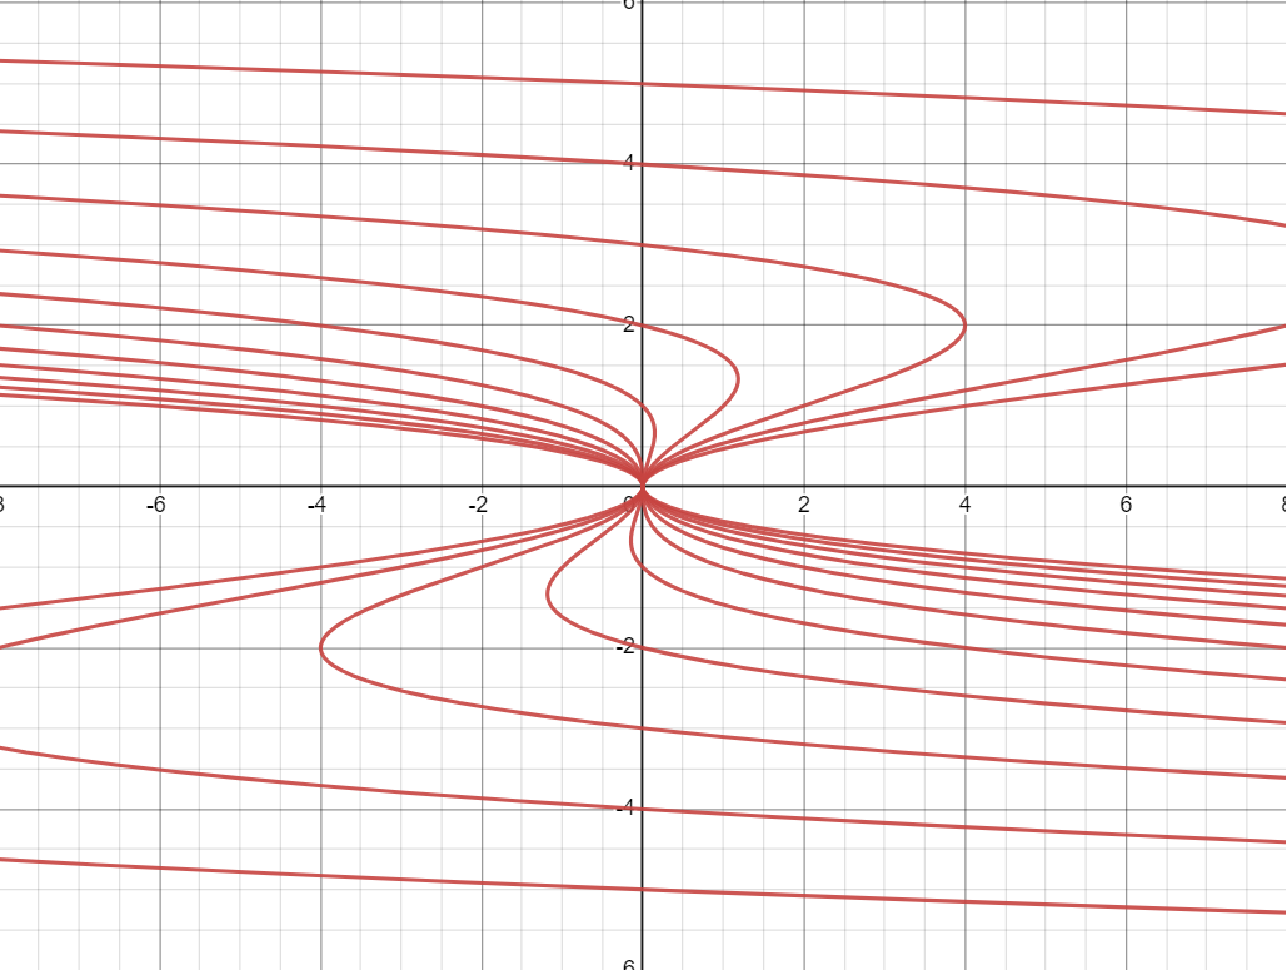
\includegraphics[width=0.5\textwidth]{figures/vec_lines_plot.pdf}
		\caption{Векторные линии поля \(\vec H\)}\label{fig:vec_lines}
	\end{figure}

\end{frame}

\subsection{Потенциал векторного поля}
\begin{frame}\frametitle{Потенциал векторного поля}
	\(U\) -- потенциал поля \(\vec H\). \\
	Возьмем одну точку с фиксированными координтатами
	$(x_0, y_0)$, а другую с переменными - $(x, y)$. \\
	Найдем потенциал по формуле:
	\begin{equation}
		U =
		\int\limits_{x_0}^{x} H_xdx + \int\limits_{y_0}^{y} H_ydy
		\label{eq:u_integral}
	\end{equation}

	\begin{align*}
		U =
		\int\limits_{x_0}^{x} 1dx -
		\int\limits_{y_0}^{y} \frac{1}{y^2} dy = 
		x - x_0 + C_1 - (-\frac{1}{y} + \frac{1}{y_0} + C_2) =
		x + \frac{1}{y} + C
	\end{align*}
	

\end{frame}
\subsection{Линии уровня потенциала}
\begin{frame}\frametitle{Линии уровня потенциала}
	Зелеными линиями изображен $x + \frac{1}{y} = C$
	\begin{figure}
		\centering
		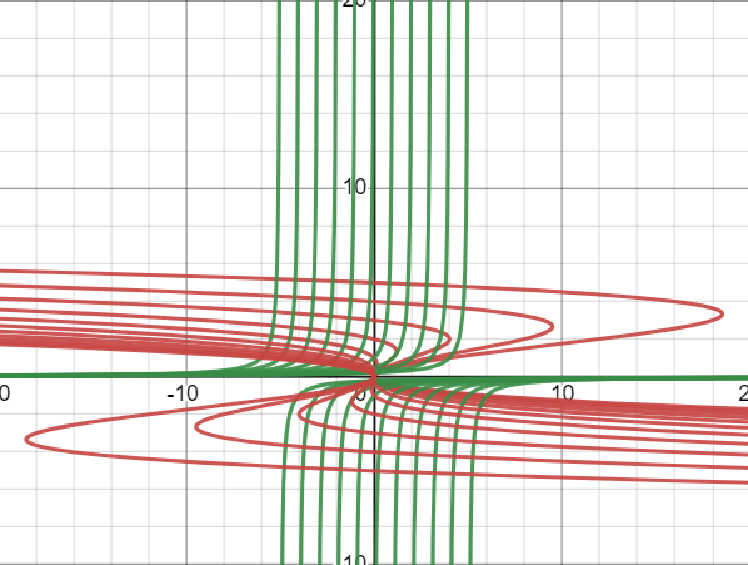
\includegraphics[width=0.5\textwidth]{figures/potential_lines_plot.pdf}
		\caption{Линии уровня потенциала поля \(\vec H\)}\label{fig:potential_lines}
	\end{figure}

\end{frame}

\subsection{Работа поля вдоль линии}
\begin{frame}\frametitle{Работа поля вдоль линии}
	За точку $A$ возьмем $(0, 1)$ за $B - (0.125, 0.5)$
	Работа поля $H$ вдоль векторной линии через это поле равна: 
	\begin{align*}
		\int\limits_{AB} \vec H \, d \vec s
		 & =
		U(B) - U(A)
		=
		(B_x + \frac{1}{B_y}) - (A_x + \frac{1}{A_y}) = \\
		 & = (0.125 + \frac{1}{0.5}) - (0 + \frac{1}{1}) = 1.125
		\label{eq:work_across_line}
	\end{align*}
	\begin{figure}
		\centering
		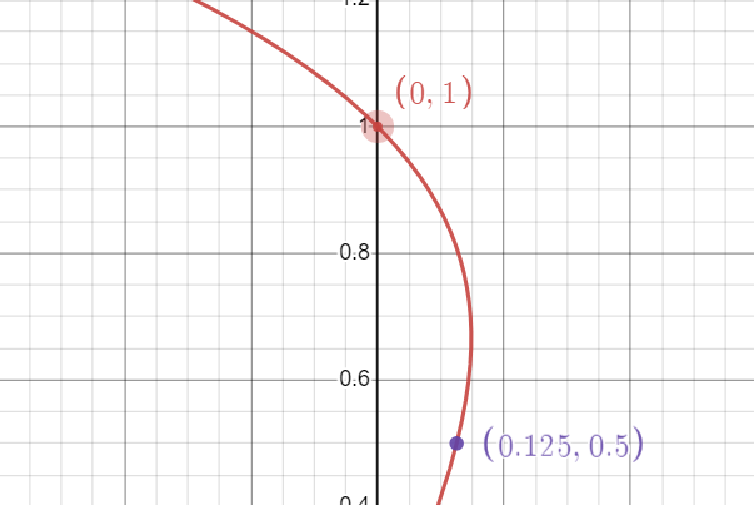
\includegraphics[width=0.5\textwidth]{figures/potential_work.pdf}
		\caption{Работа вдоль линии}\label{fig:potential_work}
	\end{figure}
\end{frame}

